\documentclass[12pt,letterpaper]{article}
\usepackage{graphicx,textcomp}
\usepackage{natbib}
\usepackage{setspace}
\usepackage{fullpage}
\usepackage{color}
\usepackage[reqno]{amsmath}
\usepackage{amsthm}
\usepackage{fancyvrb}
\usepackage{amssymb,enumerate}
\usepackage[all]{xy}
\usepackage{endnotes}
\usepackage{lscape}
\newtheorem{com}{Comment}
\usepackage{float}
\usepackage{hyperref}
\newtheorem{lem} {Lemma}
\newtheorem{prop}{Proposition}
\newtheorem{thm}{Theorem}
\newtheorem{defn}{Definition}
\newtheorem{cor}{Corollary}
\newtheorem{obs}{Observation}
\usepackage[compact]{titlesec}
\usepackage{dcolumn}
\usepackage{tikz}
\usetikzlibrary{arrows}
\usepackage{multirow}
\usepackage{xcolor}
\newcolumntype{.}{D{.}{.}{-1}}
\newcolumntype{d}[1]{D{.}{.}{#1}}
\definecolor{light-gray}{gray}{0.65}
\usepackage{url}
\usepackage{listings}
\usepackage{color}

\definecolor{codegreen}{rgb}{0,0.6,0}
\definecolor{codegray}{rgb}{0.5,0.5,0.5}
\definecolor{codepurple}{rgb}{0.58,0,0.82}
\definecolor{backcolour}{rgb}{0.95,0.95,0.92}

\lstdefinestyle{mystyle}{
	backgroundcolor=\color{backcolour},   
	commentstyle=\color{codegreen},
	keywordstyle=\color{magenta},
	numberstyle=\tiny\color{codegray},
	stringstyle=\color{codepurple},
	basicstyle=\footnotesize,
	breakatwhitespace=false,         
	breaklines=true,                 
	captionpos=b,                    
	keepspaces=true,                 
	numbers=left,                    
	numbersep=5pt,                  
	showspaces=false,                
	showstringspaces=false,
	showtabs=false,                  
	tabsize=2
}
\lstset{style=mystyle}
\newcommand{\Sref}[1]{Section~\ref{#1}}
\newtheorem{hyp}{Hypothesis}

\title{Problem Set 2}
\date{Due: October 22, 2026}
\author{Applied Stats/Quant Methods 1}
\author{Owen Stidman}

\begin{document}
	\maketitle
	\section*{Instructions}
\begin{itemize}
	\item Please show your work! You may lose points by simply writing in the answer. If the problem requires you to execute commands in \texttt{R}, please include the code you used to get your answers. Please also include the \texttt{.R} file that contains your code. If you are not sure if work needs to be shown for a particular problem, please ask.
	\item Your homework should be submitted electronically on GitHub.
	\item This problem set is due before 23:59 on Thursday October 22, 2026. No late assignments will be accepted.

\end{itemize}

	
	\vspace{.5cm}
	\section*{Question 1: Political Science}
		\vspace{.25cm}
	The following table was created using the data from a study run in a major Latin American city.\footnote{Fried, Lagunes, and Venkataramani (2010). ``Corruption and Inequality at the Crossroad: A Multimethod Study of Bribery and Discrimination in Latin America. \textit{Latin American Research Review}. 45 (1): 76-97.} As part of the experimental treatment in the study, one employee of the research team was chosen to make illegal left turns across traffic to draw the attention of the police officers on shift. Two employee drivers were upper class, two were lower class drivers, and the identity of the driver was randomly assigned per encounter. The researchers were interested in whether officers were more or less likely to solicit a bribe from drivers depending on their class (officers use phrases like, ``We can solve this the easy way'' to draw a bribe). The table below shows the resulting data.

\newpage
\begin{table}[h!]
	\centering
	\begin{tabular}{l | c c c }
		& Not Stopped & Bribe requested & Stopped/given warning \\
		\\[-1.8ex] 
		\hline \\[-1.8ex]
		Upper class & 14 & 6 & 7 \\
		Lower class & 7 & 7 & 1 \\
		\hline
	\end{tabular}
\end{table}

\begin{enumerate}
	
	\item [(a)]
	Calculate the $\chi^2$ test statistic by hand/manually (even better if you can do "by hand" in \texttt{R}).\\ 
		\lstinputlisting[language=R, firstline=40, lastline=77]{PS02_answers_OS.R} 
	
	The expected frequency for each cell is: 	\vspace{0.5cm}
	
	\textit{(row total / grand total) * column total}
	
I calculated the expected frequencies "by hand" in R (above). A table of expected frequencies is below: 
\begin{table}[h!]
	\centering
	\begin{tabular}{l | c c c }
		& Not Stopped & Bribe requested & Stopped/given warning \\
		\\[-1.8ex] 
		\hline \\[-1.8ex]
		Upper class & $f_e$ = 13.5 & $f_e$ = 8.357 & $f_e$ = 5.143 \\
		Lower class & $f_e$ = 7.5 & $f_e$ = 4.643 & $f_e$ = 2.857 \\
		\hline
	\end{tabular}
\end{table}
	
		\vspace{0.5cm}
	\item [(b)]
	Now calculate the p-value from the test statistic you just created (in \texttt{R}).\footnote{Remember frequency should be $>$ 5 for all cells, but let's calculate the p-value here anyway.}  What do you conclude if $\alpha = 0.1$?\\
	\lstinputlisting[language=R, firstline=78, lastline=113]{PS02_answers_OS.R} 
	
	The degrees of freedom for this chi-square test are: 	\vspace{0.5cm}
	
	\textit{df = (rows-1)(columns-1) = 1*2 =2} 	\vspace{0.5cm}
	
	Using the \textit{pchisq()} function in R, the chi-square statistic calculated earlier, and \textit{df = 2}, the P-value is approximately 0.15. \vspace{0.5cm}
	
	Our hypotheses are: \vspace{0.5cm}
	
	$H_0$: The socioeconomic class of the driver and whether the officer solicits a bribe from the driver are statistically independent.
	
	$H_a$: The socioeconomic class of the driver and whether the officer solicits a bribe from the driver are statistically dependent. \vspace{0.5cm}
	
	At the $alpha$ = 0.1 level, the P-value is greater than $alpha$. We \textbf{fail to reject the null hypothesis} that the socioeconomic class of the driver and whether the officer solicits a bribe from the driver are statistically independent.
	
	\newpage
	\item [(c)] Calculate the standardized residuals for each cell and put them in the table below.
	
	\begin{table}[h]
		\centering
		\begin{tabular}{l | c c c }
			& Not Stopped & Bribe requested & Stopped/given warning \\
			\\[-1.8ex] 
			\hline \\[-1.8ex]
			Upper class  & 0.322 &  -1.642 & 1.523 \\
			\\
			Lower class & -0.322 & 1.642 & -1.523  \\
			
		\end{tabular}
	\end{table}
	
\lstinputlisting[language=R, firstline=114, lastline=146]{PS02_answers_OS.R}  \vspace{0.5cm}

The standardized residual for each cell is equal to the difference in the observed and expected frequency divided by the product of the expected frequency, (1 - the row proportion), and (1 - the column proportion). That is: \vspace{0.5cm}

\textit{z} = ($f_o$ - $f_e$) / $\sqrt{f_e(1 - proportion_r)(1 - proportion_c)}$ \vspace{0.5cm}

I used the above formula manually in R and placed the results in the table above. I checked my work by calling the \textit{chisq.test()} function in R and returning the standardized residuals. The returned values were equal or approximately equal to the values I calculated by hand. Any discrepancies in the results can likely be attributed to rounding. \vspace{0.5cm}

	\item [(d)] How might the standardized residuals help you interpret the results?  \vspace{0.5cm}
	
	The standardized residuals measure the strength of each cells's contribution to the chi-square statistic (calculated earlier). Just as z-scores provide an indication of how far from the mean a given observed value of a continuous variable is, standardized residuals provide an indication of how far a categorical variable's observed frequency is from its expected frequency.
	
	If the chi-square test provided statistically significant evidence to reject the null hypothesis that the variables are statistically independent (it did not provide any such evidence in this case), the standardized residuals would indicate which cells in the contingency table (i.e., which class of driver and whether the officer requested a bribe) were driving the two variables' statistically dependent relationship. 
	
	In this case, both upper and lower class drivers who had officers request a bribe had the greatest discrepancies between the expected frequency of bribe requests and the observed frequencies. Lower class drivers had bribes requested more than expected, while upper class drivers had bribes requested less than expected. 
	
\end{enumerate}
\newpage

\section*{Question 2: Economics}
Chattopadhyay and Duflo were interested in whether women promote different policies than men.\footnote{Chattopadhyay and Duflo. (2004). ``Women as Policy Makers: Evidence from a Randomized Policy Experiment in India. \textit{Econometrica}. 72 (5), 1409-1443.} Answering this question with observational data is pretty difficult due to potential confounding problems (e.g. the districts that choose female politicians are likely to systematically differ in other aspects too). Hence, they exploit a randomized policy experiment in India, where since the mid-1990s, $\frac{1}{3}$ of village council heads have been randomly reserved for women. A subset of the data from West Bengal can be found at the following link: \url{https://raw.githubusercontent.com/kosukeimai/qss/master/PREDICTION/women.csv}\\

\noindent Each observation in the data set represents a village and there are two villages associated with one GP (i.e. a level of government is called "GP"). Figure~\ref{fig:women_desc} below shows the names and descriptions of the variables in the dataset. The authors hypothesize that female politicians are more likely to support policies female voters want. Researchers found that more women complain about the quality of drinking water than men. You need to estimate the effect of the reservation policy on the number of new or repaired drinking water facilities in the villages.
\vspace{.5cm}
\begin{figure}[h!]
	\caption{\footnotesize{Names and description of variables from Chattopadhyay and Duflo (2004).}}
	\vspace{.5cm}
	\centering
	\label{fig:women_desc}
	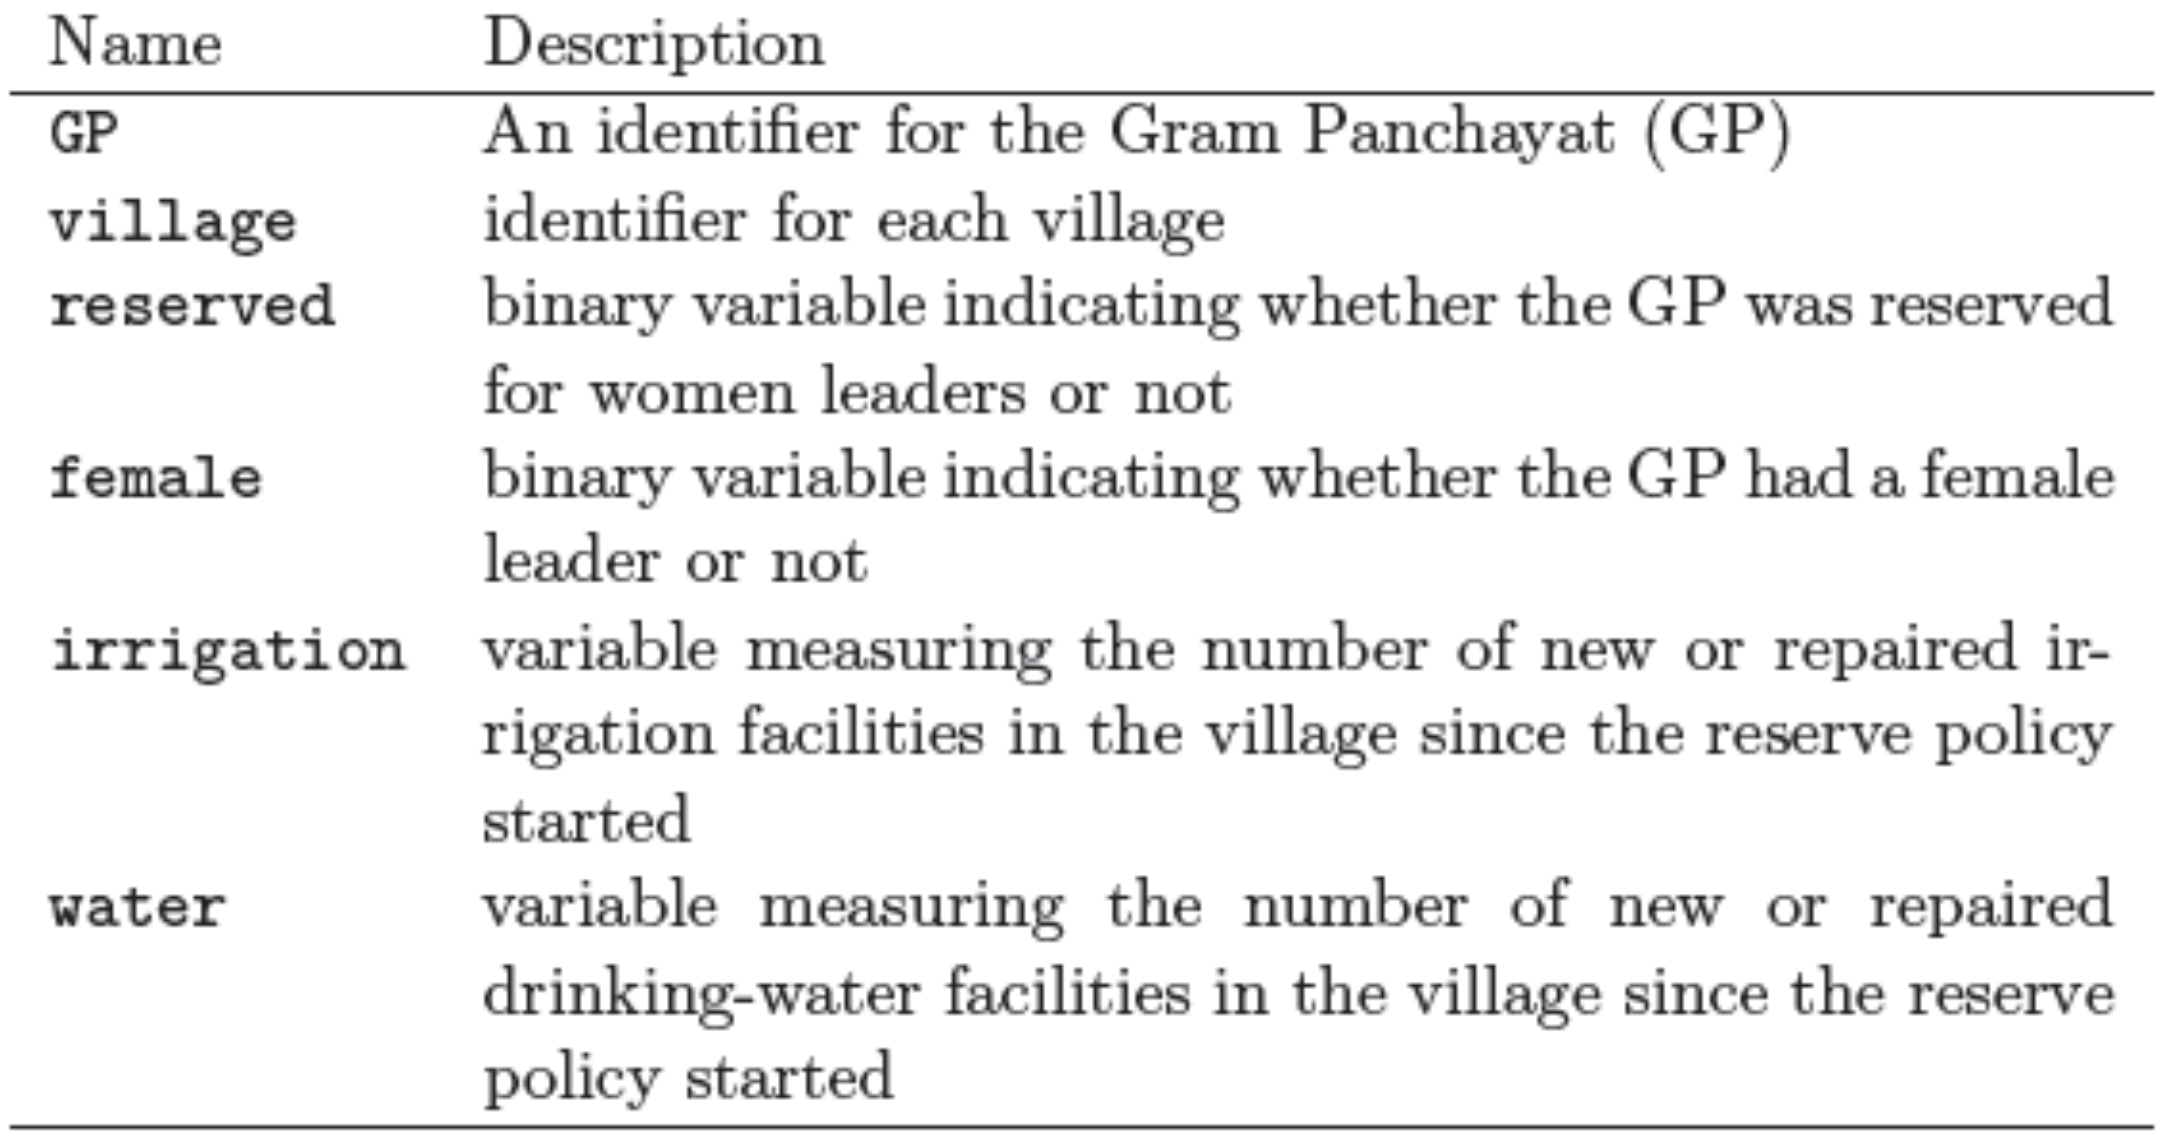
\includegraphics[scale=0.4]{duflo}
\end{figure}		

\newpage
\begin{enumerate}
	\item [(a)] State a null and alternative (two-tailed) hypothesis. 
	
	\lstinputlisting[language=R, firstline=167, lastline=168]{PS02_answers_OS.R}
	
As the question is specifically concerned with estimating the effect of the reservation policy on the number of new or repaired drinking water facilities in the villages, the two relevant variables for the bivariate regression are "reserved" (binary explanatory variable) and "water" (continuous response variable).
	
$H_0$: $\beta_1$ (slope of regression line) = 0. On average, after adopting the  reservation policy (i.e. going from "reserved = 0" to "reserved = 1"),  there is no effect on the number of new or repaired drinking water  facilities in a village. 
	
$H_a$: $\beta_1$ $\neq$ 0 On average, after adopting the  reservation policy (i.e. going from "reserved = 0" to "reserved = 1"),  there is an effect on the number of new or repaired drinking water facilities in a village. 
	
	\vspace{1cm}
	\item [(b)] Run a bivariate regression to test this hypothesis in \texttt{R} (include your code!).
	
	\lstinputlisting[language=R, firstline=188, lastline=208]{PS02_answers_OS.R} 
	
	As this problem is only concerned with two variables, I use subsetting to clean up the data so that it only includes the explanatory variable \textit{reserved} and the response variable \textit{water}. \textit{(In the interest of academic integrity, I used Google -- no AI -- to find the "select" argument for the subset() function.)}
	
	Once the data has been cleaned up, I call the \textit{lm()} function to regress the response variable \textit{water} on the explanatory variable \textit{reserved}.
	
	The \textit{lm()} function provides the following output: \vspace{0.5cm}
	
	$\hat{\beta}_0$ (intercept) = 14.738 
	
	$\hat{\beta}_1$ (slope) = 9.252
	
	\textit{se($\hat{\beta}_0$)} = 2.286
	
	\textit{se($\hat{\beta}_1$)} = 3.948
	
	\textit{t} = 2.344
	
	\textit{P}-value = 0.0197 \vspace{0.5cm}
	
	Using the $\hat{\beta}_0$ and $\hat{\beta}_1$ values above, the regression equation is: \vspace{0.5cm}
	
\textbf{	$\hat{water}$ = 14.738  +  9.252(\textit{reserved}) + $\epsilon$}

 \vspace{0.5cm}
A scatterplot of the cleaned-up data including this regression line is below, preceded by the R code used to generate the plot:
 
 	\lstinputlisting[language=R, firstline=229, lastline=243]{PS02_answers_OS.R}
	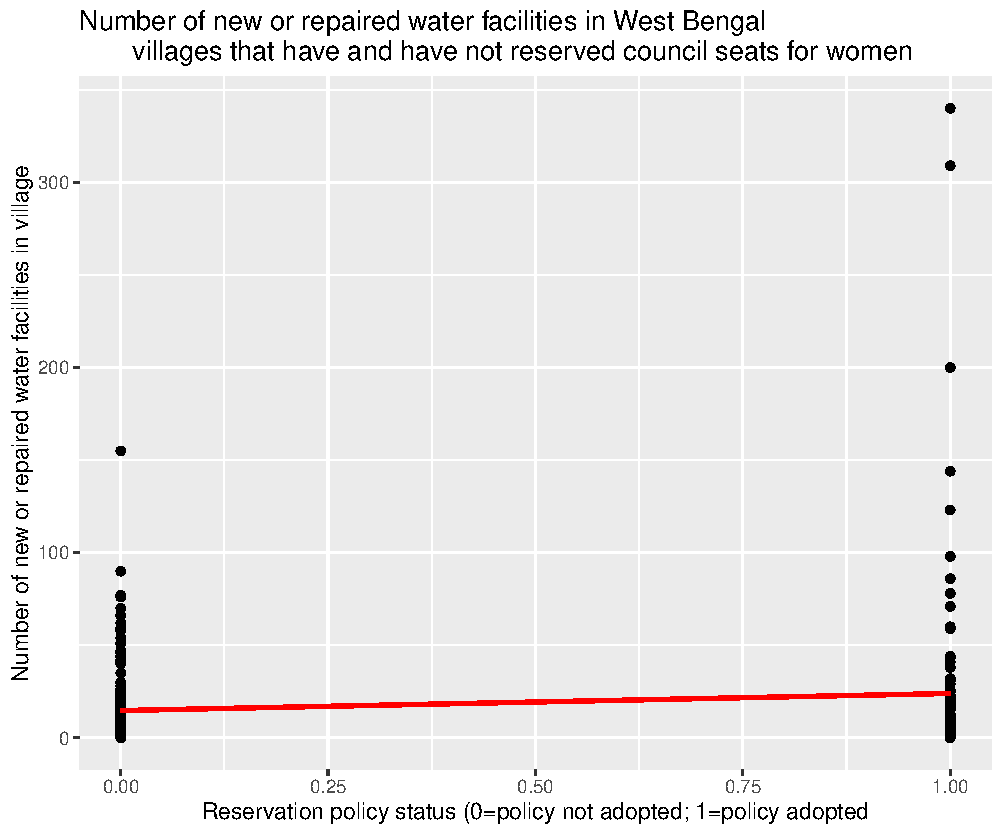
\includegraphics[scale=0.9]{scatterplot}

In checking the model assumptions, I created a residual plot in R (below, preceded by code). The residuals appear to have a heteroskedastic distribution, with the residual values for villages that have adopted the reservation policy exhibiting greater variance than those that have not adopted the reservation policy. This violates the "constant variance of error" asssumption of linear regression. A different model may be better suited for analysing this data. 

 	\lstinputlisting[language=R, firstline=245, lastline=250]{PS02_answers_OS.R}

	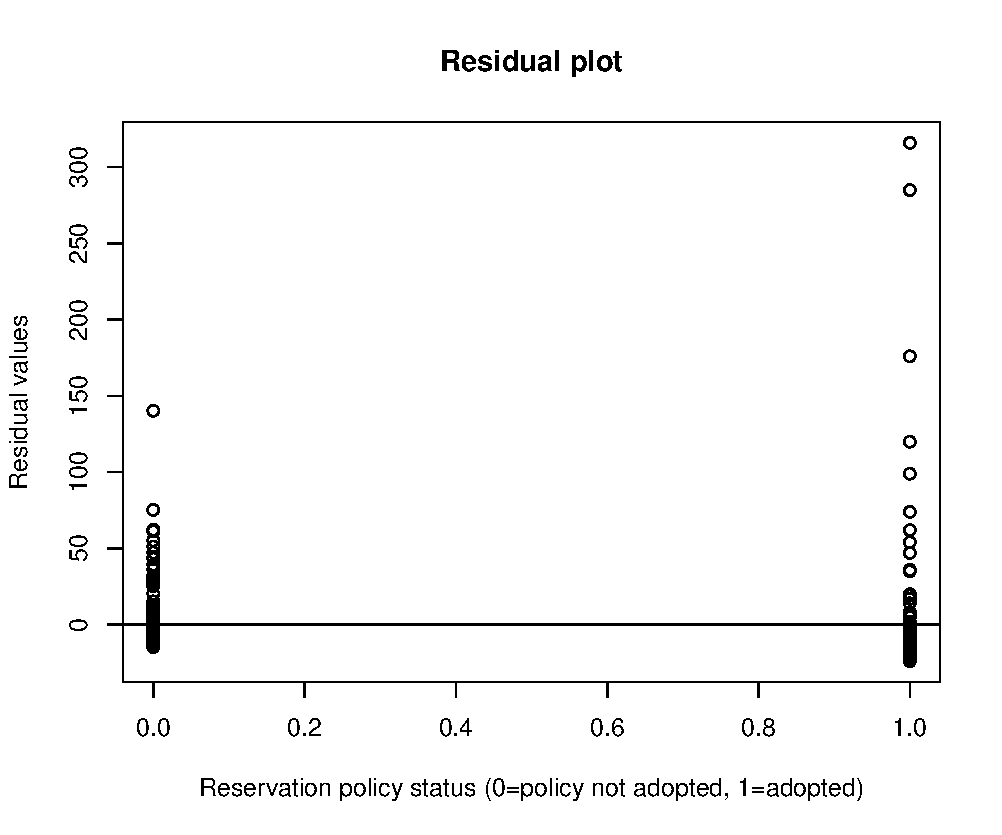
\includegraphics[scale=1]{residualplot}
	
	\vspace{1cm}
	\item [(c)] Interpret the coefficient estimate for reservation policy.  	\vspace{0.5cm}


The slope coefficient estimate $\hat{\beta}_1$ = 9.252 can be interpreted as meaning that by this model, on average, a village adopting the reservation policy (that is, going from "reserved = 0" to "reserved = 1"), would be expected to build or repair approximately 9 drinking water facilities. 
	
The P-value of 0.0197 is less than $\alpha$ = 0.05. At the $\alpha$ = 0.05 level, we can \textbf{reject the null hypothesis} that after adopting the reservation policy (i.e. going from "reserved = 0" to "reserved = 1"), there is no effect on the number of new or repaired drinking water facilities in a village. The slope of the linear regression line is statistically different from zero.
\end{enumerate}


%\end{enumerate}
\end{document}
